%%%%%%%%%%%%%%%%%%%%%%%%%%%%%%%%%%
%%%%%%%%%%%%%%%%%%%%%%%%%%%%%%%%%%
%Plantilla pel Treball Fi de Grau
%%%%%%%%%%%%%%%%%%%%%%%%%%%%%%%%%%
%%%%%%%%%%%%%%%%%%%%%%%%%%%%%%%%%%%%%%%%%%%
\documentclass[twocolumn]{revtex4}
%%%%%%%%%%%%%%%%%%%%%%%%%%%%%%%%%%%%%%%%%%%
\usepackage{graphicx,epsfig}
\usepackage{amsmath}
\usepackage{amsfonts}

\usepackage{fancyhdr}

%%%%%%%%%%%%%%%%%%%%%%%%%%%%%%%%%%%%%%%%%%%
%%%%%%%%%%%%%%%%%%%%%%%%%%%%%%%%%%%%%%%%%%%


\begin{document}


%%%%%%%%%%%%%%%%%%%%%%%%%%%%%%%%%%%%%%

%Això és un comentari que no surt al text.

%%%%%%%%%%%%%%%%%%%%%%%%%%%%%%%%%%%%%%
%Es pot ometre
\pagestyle{fancy}
\lhead{\bf TITLE}
\rhead{Student's name}
\lfoot{Treball de Fi de Grau}
\rfoot{Barcelona, March 2022}
%%%%%%%%%%%%%%%%%%%%%%%%%%%%%%%%%%%%%%


\title{Evaluation of the performance of $\Delta \phi$ as a precipitation estimator}
\author{Author: Ignacio Cordova Pou}
\affiliation{Facultat de F\'{\i}sica, Universitat de Barcelona, Diagonal
645, 08028 Barcelona, Spain.}
%\email{tfgac@ub.edu} %optional
\author{Advisor: Dr. Ramon Padullès}
\date{\today}

\begin{abstract}
{\bf Abstract:}
This paper introduces the application of statistical models 
to determine the performance of the observable $\Delta \phi$
as a precipitation estimator. Using Precision Recall curves, the 
study shows the optimal range of heights for transforming the vertical 
profiles of $\Delta\phi$ into a scalar average. The results show 
that Using NASA's IMERG precipitation data as our target with the 
97th percentile mm/h as True, $\Delta\phi$ achievesan optimal F1 score 
of 0.54 when averaged between 0.1km and 8.5km. 

\end{abstract}

\maketitle

%\tableofcontents

%%%%%%%%%%%%%%%%%%%%%%%%%%%%%%%%%%%%%%%%%%%%%%%%%%%%%%%%%%%%%%%%%%%%%%%%%%%
\section{Introduction}

A Global Navigation Satellite System (GNSS) radio 
occultation (RO) experiment is taking place in the Spanish 
low Earth orbiter PAZ satellite. The RO payload provides
globally distributed vertical profiles of 
the atmosphere which have been proven to have a high impact on Numerical Weather
Prediction Models[referencia]. Moreover, the mission runs for the first
time a double-polarization GNSS RO experiment for detecting precipitation
events. The performance of this new technique, which has already been 
proven to be succesfull, is evaluated in this paper.

The GNSS systems transmit circular-polarized signals that are collected 
using ROs after having travelled through the atmosphere. 
They are collected using two orthogonal linearly polarized antennas 
(horizontal H and vertical V) with the aim of comparing the phase
delay $\phi_H$ and $\phi_V$. In the case of heavy rain events,
water drops experience
air friction which causes them to flatten out along their horizontal 
dimension. The pressence of water drops can cause depolarization
between the H and V signals which are affected differently when 
propagating through a rainy atmosphere. The polarimetric radio occultations (PROs) is a 
new technique that allows us to measure the differential phase shift $\Delta \phi$
between the H and V signals. One of the objectives of 
the ROHP-PAZ mission is to use the measured depolarization $\Delta \phi$ 
as a precipitation estimator.

This paper evaluates the performance of $\Delta \phi$  on 
detecting precipitation events. To properly evaluate the performance 
a target must be defined. The target used in this paper
is the NASA's IMERG precipitation dataset. From this dataset we can obtain 
the precipitation in mm/h at every location in time and space where our 
PROs took place. The goal is to evaluate and quantify how well does 
the $\Delta \phi$ estimator perform in detecting precipitation above a certain
threshold regarded as {\it true precipitation}. This way, {\bf our target 
is defined as a binary True/False variable} being True for precipitation
above the elected threshold and False for precipitation below it. 

Our array-like observable is of little use to the Numerical Weather
Prediction Models. This study provides the optimal range of heights 
$[h_o, h_f]$ for transforming the vertical profiles of $\Delta\phi$ into a scalar 
average. This optimal range depends on the threshold used to binarize 
our {\it true precipitation} and, as found in this study, on the region where
the PRO took place. The performance of each average $[h_o, h_f]$ is evaluated
using Precision-Recall curves which have been proven to 
work well with unbalanced datasets [reference]. In our case, the target
False (no precipitation event) will outnumber the target True once a proper
truth threshold is defined. 

It is expected that the average $[h_o, h_f]$ that best predicts the 
True/False target will be somewhere between 0.1km and 10.0km since that 
is where the signal will experiment the most depolarization. 

%%%%%%%%%%%%%%%%%%%%%%%%%%%%%%%%%%%%%%%%%%%%%%%%%%%%%%%%%%%%%%%%%%%%%%%%%
\section{Data}

The data collected by the PAZ satellite are downlinked by Hisdesat.
The Institut de Ciències de l'Espai (ICE), Consejo Superior de Investigaciones
Científicas, Institut d'Estudis Espacials de Catalunya (CSIC, IEEC) collects 
and owns the data and provides access to the servers at the Jet Propulsion 
Laboratory (JPL). At the JPL, the raw data are processed and converted to 
level 1 RO products, which are finally analyzed.

The main observable of the experiment is the differential phase shift
\begin{equation}
    \Delta \phi =\phi_H - \phi_V,
\label{eq:1}
\end{equation}
The dataset is composed of over 85.000 measurements distributed globally 
providing vertical profiles of $\Delta\phi$  in 100m intervals between
0.1km and 40km. A {\it true precipitation} is associated with each of 
these measurements. As an example, 1 measurement is shown below: 
\begin{figure}[h!]
\centering
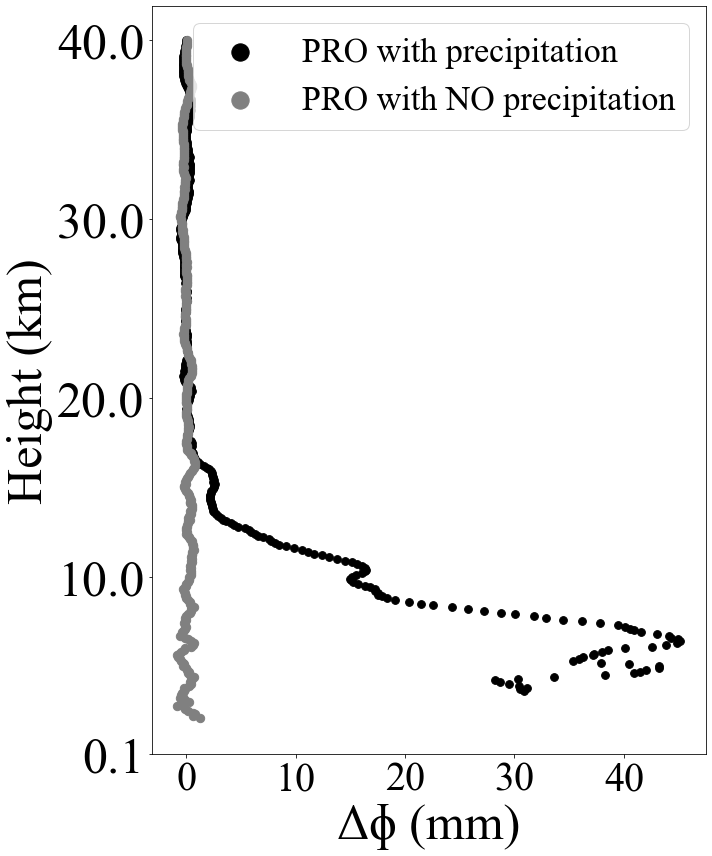
\includegraphics[scale=0.3]{vprofile.png}
\caption{A sample figure.}
\label{fig:sample}
\end{figure}




You can insert equations in the text, like $e^{i \pi} +1=0$;
$\frac{df(x)}{dx}$ or you may prefer
$\displaystyle \frac{df(x)}{dx}$.
You can also write aligned equations,
\begin{eqnarray}
\frac{du(x)}{dx}+V u(x) +W v(x) &=& (\lambda + \alpha)  \; u(x) \nonumber \\
\frac{dv(x)}{dx}+V v(x) +W u(x) &=& (\lambda - \alpha) \; v(x).
\label{eq:tercera}\end{eqnarray}
Further examples are,
\begin{eqnarray}
\nabla {\cdot} \vec{E}&=& 4 \pi \rho \nonumber \\
\nabla \times \vec{B} - \frac{1}{c} \frac{\partial \vec{E}}{\partial t} &=&
\frac{4 \pi}{c} \vec{J} \nonumber \\
\nabla \times \vec{E} +\frac{1}{c} \frac{\partial \vec{B}}{\partial t} &=&
0 \nonumber \\
\nabla {\cdot} \vec{E}&=& 0,
\label{maxwell}
\end{eqnarray}
as can be found in \cite{jackson}, pag. 14. Also,
\begin{equation}
E = -J \sum_{i=1}^N s_i s_{i+1}.
\label{eq:ising}
\end{equation}

You can define your own macros to save typing
\footnote{This is a footnote.}.
For example, suppose
that you introduce a macro as follows:
\newcommand{\El}{{\vec{E}(\vec{x},t)}}
\begin{verbatim}
\newcommand{\El}{{\vec{E}(\vec{x},t)}}
\end{verbatim}
Then, by simply typing,
\begin{verbatim}
$\El$
\end{verbatim}
you get the electric field $\El$ printed out (in math mode, of course).

\vspace*{0.5cm}
You can write $\tilde x$,
$\overline{A}$; \%, accents: Schr\"odinger
and \'e, \`a, \`A, Mart\'{\i}; cal\c cotada,
$A \equiv B $, $\vec{A}\cdot\vec{B}$, $\vec{A} \times \vec{B}$,
$\vec{v}$, $\hat{n}$,
$c \sim d$, $z \approx w$, $\langle x \rangle$,
$\langle \psi | X | \psi \rangle$, $\hbar$, $g_{ij}$, $\delta^i_j$,
$R_{\mu \nu \alpha \beta ; \xi}$.

\vspace*{0.5cm}
You can also quote references easily, i.e., \cite{wmap}, \cite{weinberg}.

\vspace*{0.5cm}
A matrix
\begin{equation}
\left(
\begin{array}{ccc}
0 & 1 & 0 \\
1 & 0 & 1 \\
0 & 1 & 0
\end{array}
\right),
\label{matrix1}
\end{equation}
a vector (column)
\begin{equation}
\left(
\begin{array}{c}
1 \\
\sqrt{3}\\
\pi
\end{array}
\right),
\label{hola}
\end{equation}
a row,
\begin{equation}
\left(
\begin{array}{ccc}
p & q & r
\end{array}
\right),
\label{eq:row}
\end{equation}
and a determinant,
\begin{equation}
\left|
\begin{array}{ccc}
a_{11} & a_{12} & a_{13} \\
a_{21} & a_{22} & a_{23} \\
a_{31} & a_{32} & a_{33}
\end{array}
\right|.
\label{determinant}
\end{equation}

\noindent
Further examples:
\begin{equation}
\int_{-\infty}^\infty e^{-x^2} \, dx= \sqrt{\pi},
\label{eq:fine}
\end{equation}
also,
\begin{equation}
\int_a^b f'(x) \; dx=f(b)-f(a),
\label{barrow}
\end{equation}
and so on.

\subsection{Tables and figures}

An example of a table is shown in Table~\ref{tab:sample1}.

\begin{table}[h!]
\centering
\caption{Force, area, and pressure data for an experiment with glass syringes.}
\label{tab:sample1}
\vspace*{2mm}
\begin{tabular}{|l|l|l|}
\hline
& Piston 1 & Piston 2 \\
\hline
Force\,(N) & 4.40 & 2.25 \\
Area\,(cm$^2$) & 6.16 & 3.14 \\
Pressure\,(N/cm$^2$) & $0.714 \pm 0.002$ & 0.716 \\
\hline
\end{tabular}
\end{table}

Here we try to insert an ilustrating figure, Fig.~\ref{fig:sample}.
For that you need to have created the figure before, in this case
the fig1.pdf file.

\begin{figure}[h!]
\centering
\includegraphics[width=\columnwidth]{fig1.pdf}
\caption{A sample figure.}
\label{fig:sample}
\end{figure}

%%%%%%%%%%%%%%%%%%%%%%%%%%%%%%%%%%%%%%%%%%%%%%%%%%%%%%%%%%%%%%%%%%%%%%%%
\section{Developing sections}
. . . . . . . . . . . . . . . . . . . . . . . . . . . . . . . . . . . . . . . .
. . . . . . . . . . . . . . . . . . . . . . . . . . . . . . . . . . . . . . . .
. . . . . . . . . . . . . . . . . . . . . . . . . . . . . . . . . . . . . . . .
. . . . . . . . . . . . . . . . . . . . . . . . . . . . . . . . . . . . . . . .
. . . . . . . . . . . . . . . . . . . . . . . . . . . . . . . . . . . . . . . .
. . . . . . . . . . . . . . . . . . . . . . . . . . . . . . . . . . . . . . . .
. . . . . . . . . . . . . . . . . . . . . . . . . . . . . . . . . . . . . . . .
. . . . . . . . . . . . . . . . . . . . . . . . . . . . . . . . . . . . . . . .
. . . . . . . . . . . . . . . . . . . . . . . . . . . . . . . . . . . . . . . .
. . . . . . . . . . . . . . . . . . . . . . . . . . . . . . . . . . . . . . . .
. . . . . . . . . . . . . . . . . . . . . . . . . . . . . . . . . . . . . . . .
. . . . . . . . . . . . . . . . . . . . . . . . . . . . . . . . . . . . . . . .
. . . . . . . . . . . . . . . . . . . . . . . . . . . . . . . . . . . . . . . .
. . . . . . . . . . . . . . . . . . . . . . . . . . . . . . . . . . . . . . . .
. . . . . . . . . . . . . . . . . . . . . . . . . . . . . . . . . . . . . . . .
. . . . . . . . . . . . . . . . . . . . . . . . . . . . . . . . . . . . . . . .
. . . . . . . . . . . . . . . . . . . . . . . . . . . . . . . . . . . . . . . .
. . . . . . . . . . . . . . . . . . . . . . . . . . . . . . . . . . . . . . . .
. . . . . . . . . . . . . . . . . . . . . . . . . . . . . . . . . . . . . . . .
. . . . . . . . . . . . . . . . . . . . . . . . . . . . . . . . . . . . . . . .
. . . . . . . . . . . . . . . . . . . . . . . . . . . . . . . . . . . . . . . .
. . . . . . . . . . . . . . . . . . . . . . . . . . . . . . . . . . . . . . . .
. . . . . . . . . . . . . . . . . . . . . . . . . . . . . . . . . . . . . . . .
. . . . . . . . . . . . . . . . . . . . . . . . . . . . . . . . . . . . . . . .
. . . . . . . . . . . . . . . . . . . . . . . . . . . . . . . . . . . . . . . .
. . . . . . . . . . . . . . . . . . . . . . . . . . . . . . . . . . . . . . . .
. . . . . . . . . . . . . . . . . . . . . . . . . . . . . . . . . . . . . . . .
. . . . . . . . . . . . . . . . . . . . . . . . . . . . . . . . . . . . . . . .
. . . . . . . . . . . . . . . . . . . . . . . . . . . . . . . . . . . . . . . .
. . . . . . . . . . . . . . . . . . . . . . . . . . . . . . . . . . . . . . . .
. . . . . . . . . . . . . . . . . . . . . . . . . . . . . . . . . . . . . . . .
. . . . . . . . . . . . . . . . . . . . . . . . . . . . . . . . . . . . . . . .
. . . . . . . . . . . . . . . . . . . . . . . . . . . . . . . . . . . . . . . .
. . . . . . . . . . . . . . . . . . . . . . . . . . . . . . . . . . . . . . . .
. . . . . . . . . . . . . . . . . . . . . . . . . . . . . . . . . . . . . . . .
. . . . . . . . . . . . . . . . . . . . . . . . . . . . . . . . . . . . . . . .
. . . . . . . . . . . . . . . . . . . . . . . . . . . . . . . . . . . . . . . .
. . . . . . . . . . . . . . . . . . . . . . . . . . . . . . . . . . . . . . . .
. . . . . . . . . . . . . . . . . . . . . . . . . . . . . . . . . . . . . . . .

\begin{table}[h!]
\centering
\caption{Another table.}
\label{tab:sample2}
\vspace*{2mm}
\begin{tabular}{||c||l|l|l||} \hline \hline
{\bf M1}  & Teoria:      & Galileo         & A11G \\ \cline{2-4}
 (11:45)  & Problemes:   & Newton          & A11G \\ \cline{1-4}
          & Problemes    & Planck (M1A)    & A11G \\ \cline{3-4}
 (12:45)  & tutoritzats: & Fermi (M1B)     & A23M \\
\hline \hline
{\bf M2}  & Teoria:      & Clausius        & A12G \\ \cline{2-4}
 (8:30)   & Problemes:   & Goeppert Mayer  & A12G \\ \cline{1-4}
          & Problemes    & Boltzmann (M2A) & A12G \\ \cline{3-4}
 (9:30)   & tutoritzats: & Maxwell (M2B)   & A24M \\
\hline \hline
{\bf T1}  & Teoria:      & Gibbs           & A12G \\ \cline{2-4}
 (18:00)  & Problemes:   & Helmholtz       & A12G \\ \cline{1-4}
          & Problemes    & Bohr (T1A)      & A12G \\ \cline{3-4}
 (19:00)  & tutoritzats: & Einstein (T1B)  & A24M \\
\hline \hline
\end{tabular}
\end{table}

\vspace*{0.5cm}

. . . . . . . . . . . . . . . . . . . . . . . . . . . . . . . . . . . . . . . .
. . . . . . . . . . . . . . . . . . . . . . . . . . . . . . . . . . . . . . . .
. . . . . . . . . . . . . . . . . . . . . . . . . . . . . . . . . . . . . . . .
. . . . . . . . . . . . . . . . . . . . . . . . . . . . . . . . . . . . . . . .
. . . . . . . . . . . . . . . . . . . . . . . . . . . . . . . . . . . . . . . .
. . . . . . . . . . . . . . . . . . . . . . . . . . . . . . . . . . . . . . . .
. . . . . . . . . . . . . . . . . . . . . . . . . . . . . . . . . . . . . . . .
. . . . . . . . . . . . . . . . . . . . . . . . . . . . . . . . . . . . . . . .
. . . . . . . . . . . . . . . . . . . . . . . . . . . . . . . . . . . . . . . .
. . . . . . . . . . . . . . . . . . . . . . . . . . . . . . . . . . . . . . . .
. . . . . . . . . . . . . . . . . . . . . . . . . . . . . . . . . . . . . . . .
. . . . . . . . . . . . . . . . . . . . . . . . . . . . . . . . . . . . . . . .
. . . . . . . . . . . . . . . . . . . . . . . . . . . . . . . . . . . . . . . .
. . . . . . . . . . . . . . . . . . . . . . . . . . . . . . . . . . . . . . . .
. . . . . . . . . . . . . . . . . . . . . . . . . . . . . . . . . . . . . . . .
. . . . . . . . . . . . . . . . . . . . . . . . . . . . . . . . . . . . . . . .
. . . . . . . . . . . . . . . . . . . . . . . . . . . . . . . . . . . . . . . .
. . . . . . . . . . . . . . . . . . . . . . . . . . . . . . . . . . . . . . . .
. . . . . . . . . . . . . . . . . . . . . . . . . . . . . . . . . . . . . . . .
. . . . . . . . . . . . . . . . . . . . . . . . . . . . . . . . . . . . . . . .
. . . . . . . . . . . . . . . . . . . . . . . . . . . . . . . . . . . . . . . .
. . . . . . . . . . . . . . . . . . . . . . . . . . . . . . . . . . . . . . . .
. . . . . . . . . . . . . . . . . . . . . . . . . . . . . . . . . . . . . . . .
. . . . . . . . . . . . . . . . . . . . . . . . . . . . . . . . . . . . . . . .
. . . . . . . . . . . . . . . . . . . . . . . . . . . . . . . . . . . . . . . .
. . . . . . . . . . . . . . . . . . . . . . . . . . . . . . . . . . . . . . . .
. . . . . . . . . . . . . . . . . . . . . . . . . . . . . . . . . . . . . . . .
. . . . . . . . . . . . . . . . . . . . . . . . . . . . . . . . . . . . . . . .
. . . . . . . . . . . . . . . . . . . . . . . . . . . . . . . . . . . . . . . .
. . . . . . . . . . . . . . . . . . . . . . . . . . . . . . . . . . . . . . . .
. . . . . . . . . . . . . . . . . . . . . . . . . . . . . . . . . . . . . . . .
. . . . . . . . . . . . . . . . . . . . . . . . . . . . . . . . . . . . . . . .
. . . . . . . . . . . . . . . . . . . . . . . . . . . . . . . . . . . . . . . .
. . . . . . . . . . . . . . . . . . . . . . . . . . . . . . . . . . . . . . . .
. . . . . . . . . . . . . . . . . . . . . . . . . . . . . . . . . . . . . . . .
. . . . . . . . . . . . . . . . . . . . . . . . . . . . . . . . . . . . . . . .
. . . . . . . . . . . . . . . . . . . . . . . . . . . . . . . . . . . . . . . .
. . . . . . . . . . . . . . . . . . . . . . . . . . . . . . . . . . . . . . . .
. . . . . . . . . . . . . . . . . . . . . . . . . . . . . . . . . . . . . . . .
. . . . . . . . . . . . . . . . . . . . . . . . . . . . . . . . . . . . . . . .
. . . . . . . . . . . . . . . . . . . . . . . . . . . . . . . . . . . . . . . .
. . . . . . . . . . . . . . . . . . . . . . . . . . . . . . . . . . . . . . . .
. . . . . . . . . . . . . . . . . . . . . . . . . . . . . . . . . . . . . . . .
. . . . . . . . . . . . . . . . . . . . . . . . . . . . . . . . . . . . . . . .
. . . . . . . . . . . . . . . . . . . . . . . . . . . . . . . . . . . . . . . .
. . . . . . . . . . . . . . . . . . . . . . . . . . . . . . . . . . . . . . . .
. . . . . . . . . . . . . . . . . . . . . . . . . . . . . . . . . . . . . . . .
. . . . . . . . . . . . . . . . . . . . . . . . . . . . . . . . . . . . . . . .
. . . . . . . . . . . . . . . . . . . . . . . . . . . . . . . . . . . . . . . .
. . . . . . . . . . . . . . . . . . . . . . . . . . . . . . . . . . . . . . . .
. . . . . . . . . . . . . . . . . . . . . . . . . . . . . . . . . . . . . . . .
. . . . . . . . . . . . . . . . . . . . . . . . . . . . . . . . . . . . . . . .
. . . . . . . . . . . . . . . . . . . . . . . . . . . . . . . . . . . . . . . .
. . . . . . . . . . . . . . . . . . . . . . . . . . . . . . . . . . . . . . . .
. . . . . . . . . . . . . . . . . . . . . . . . . . . . . . . . . . . . . . . .
. . . . . . . . . . . . . . . . . . . . . . . . . . . . . . . . . . . . . . . .
. . . . . . . . . . . . . . . . . . . . . . . . . . . . . . . . . . . . . . . .
. . . . . . . . . . . . . . . . . . . . . . . . . . . . . . . . . . . . . . . .
. . . . . . . . . . . . . . . . . . . . . . . . . . . . . . . . . . . . . . . .
. . . . . . . . . . . . . . . . . . . . . . . . . . . . . . . . . . . . . . . .
. . . . . . . . . . . . . . . . . . . . . . . . . . . . . . . . . . . . . . . .
. . . . . . . . . . . . . . . . . . . . . . . . . . . . . . . . . . . . . . . .
. . . . . . . . . . . . . . . . . . . . . . . . . . . . . . . . . . . . . . . .
. . . . . . . . . . . . . . . . . . . . . . . . . . . . . . . . . . . . . . . .
. . . . . . . . . . . . . . . . . . . . . . . . . . . . . . . . . . . . . . . .
. . . . . . . . . . . . . . . . . . . . . . . . . . . . . . . . . . . . . . . .
. . . . . . . . . . . . . . . . . . . . . . . . . . . . . . . . . . . . . . . .
. . . . . . . . . . . . . . . . . . . . . . . . . . . . . . . . . . . . . . . .
. . . . . . . . . . . . . . . . . . . . . . . . . . . . . . . . . . . . . . . .
. . . . . . . . . . . . . . . . . . . . . . . . . . . . . . . . . . . . . . . .
. . . . . . . . . . . . . . . . . . . . . . . . . . . . . . . . . . . . . . . .
. . . . . . . . . . . . . . . . . . . . . . . . . . . . . . . . . . . . . . . .
. . . . . . . . . . . . . . . . . . . . . . . . . . . . . . . . . . . . . . . .
. . . . . . . . . . . . . . . . . . . . . . . . . . . . . . . . . . . . . . . .
. . . . . . . . . . . . . . . . . . . . . . . . . . . . . . . . . . . . . . . .
. . . . . . . . . . . . . . . . . . . . . . . . . . . . . . . . . . . . . . . .
. . . . . . . . . . . . . . . . . . . . . . . . . . . . . . . . . . . . . . . .
. . . . . . . . . . . . . . . . . . . . . . . . . . . . . . . . . . . . . . . .
. . . . . . . . . . . . . . . . . . . . . . . . . . . . . . . . . . . . . . . .
. . . . . . . . . . . . . . . . . . . . . . . . . . . . . . . . . . . . . . . .
. . . . . . . . . . . . . . . . . . . . . . . . . . . . . . . . . . . . . . . .
. . . . . . . . . . . . . . . . . . . . . . . . . . . . . . . . . . . . . . . .
. . . . . . . . . . . . . . . . . . . . . . . . . . . . . . . . . . . . . . . .
. . . . . . . . . . . . . . . . . . . . . . . . . . . . . . . . . . . . . . . .
. . . . . . . . . . . . . . . . . . . . . . . . . . . . . . . . . . . . . . . .
. . . . . . . . . . . . . . . . . . . . . . . . . . . . . . . . . . . . . . . .
. . . . . . . . . . . . . . . . . . . . . . . . . . . . . . . . . . . . . . . .
. . . . . . . . . . . . . . . . . . . . . . . . . . . . . . . . . . . . . . . .
. . . . . . . . . . . . . . . . . . . . . . . . . . . . . . . . . . . . . . . .
. . . . . . . . . . . . . . . . . . . . . . . . . . . . . . . . . . . . . . . .
. . . . . . . . . . . . . . . . . . . . . . . . . . . . . . . . . . . . . . . .
. . . . . . . . . . . . . . . . . . . . . . . . . . . . . . . . . . . . . . . .
. . . . . . . . . . . . . . . . . . . . . . . . . . . . . . . . . . . . . . . .
. . . . . . . . . . . . . . . . . . . . . . . . . . . . . . . . . . . . . . . .
. . . . . . . . . . . . . . . . . . . . . . . . . . . . . . . . . . . . . . . .
. . . . . . . . . . . . . . . . . . . . . . . . . . . . . . . . . . . . . . . .
. . . . . . . . . . . . . . . . . . . . . . . . . . . . . . . . . . . . . . . .
. . . . . . . . . . . . . . . . . . . . . . . . . . . . . . . . . . . . . . . .
. . . . . . . . . . . . . . . . . . . . . . . . . . . . . . . . . . . . . . . .
. . . . . . . . . . . . . . . . . . . . . . . . . . . . . . . . . . . . . . . .
. . . . . . . . . . . . . . . . . . . . . . . . . . . . . . . . . . . . . . . .
. . . . . . . . . . . . . . . . . . . . . . . . . . . . . . . . . . . . . . . .
. . . . . . . . . . . . . . . . . . . . . . . . . . . . . . . . . . . . . . . .
. . . . . . . . . . . . . . . . . . . . . . . . . . . . . . . . . . . . . . . .
. . . . . . . . . . . . . . . . . . . . . . . . . . . . . . . . . . . . . . . .
. . . . . . . . . . . . . . . . . . . . . . . . . . . . . . . . . . . . . . . .
. . . . . . . . . . . . . . . . . . . . . . . . . . . . . . . . . . . . . . . .

\subsection{Subsection 1}

This is the first subsection.
\begin{figure}[h!]
\centering
\includegraphics[width=6.0cm]{fig1.pdf}
\caption{A sample figure made smaller by changing the width parameter.}
\label{fig:small_sample}
\end{figure}



\vspace*{0.5cm}
\noindent
. . . . . . . . . . . . . . . . . . . . . . . . . . . . . . . . . . . . . . . .
. . . . . . . . . . . . . . . . . . . . . . . . . . . . . . . . . . . . . . . .
. . . . . . . . . . . . . . . . . . . . . . . . . . . . . . . . . . . . . . . .
. . . . . . . . . . . . . . . . . . . . . . . . . . . . . . . . . . . . . . . .
. . . . . . . . . . . . . . . . . . . . . . . . . . . . . . . . . . . . . . . .
. . . . . . . . . . . . . . . . . . . . . . . . . . . . . . . . . . . . . . . .
. . . . . . . . . . . . . . . . . . . . . . . . . . . . . . . . . . . . . . . .
. . . . . . . . . . . . . . . . . . . . . . . . . . . . . . . . . . . . . . . .
. . . . . . . . . . . . . . . . . . . . . . . . . . . . . . . . . . . . . . . .
. . . . . . . . . . . . . . . . . . . . . . . . . . . . . . . . . . . . . . . .
. . . . . . . . . . . . . . . . . . . . . . . . . . . . . . . . . . . . . . . .
. . . . . . . . . . . . . . . . . . . . . . . . . . . . . . . . . . . . . . . .
. . . . . . . . . . . . . . . . . . . . . . . . . . . . . . . . . . . . . . . .
. . . . . . . . . . . . . . . . . . . . . . . . . . . . . . . . . . . . . . . .
. . . . . . . . . . . . . . . . . . . . . . . . . . . . . . . . . . . . . . . .
. . . . . . . . . . . . . . . . . . . . . . . . . . . . . . . . . . . . . . . .
. . . . . . . . . . . . . . . . . . . . . . . . . . . . . . . . . . . . . . . .
. . . . . . . . . . . . . . . . . . . . . . . . . . . . . . . . . . . . . . . .
. . . . . . . . . . . . . . . . . . . . . . . . . . . . . . . . . . . . . . . .
. . . . . . . . . . . . . . . . . . . . . . . . . . . . . . . . . . . . . . . .
. . . . . . . . . . . . . . . . . . . . . . . . . . . . . . . . . . . . . . . .
. . . . . . . . . . . . . . . . . . . . . . . . . . . . . . . . . . . . . . . .
. . . . . . . . . . . . . . . . . . . . . . . . . . . . . . . . . . . . . . . .
. . . . . . . . . . . . . . . . . . . . . . . . . . . . . . . . . . . . . . . .
. . . . . . . . . . . . . . . . . . . . . . . . . . . . . . . . . . . . . . . .
. . . . . . . . . . . . . . . . . . . . . . . . . . . . . . . . . . . . . . . .
. . . . . . . . . . . . . . . . . . . . . . . . . . . . . . . . . . . . . . . .
. . . . . . . . . . . . . . . . . . . . . . . . . . . . . . . . . . . . . . . .
. . . . . . . . . . . . . . . . . . . . . . . . . . . . . . . . . . . . . . . .
. . . . . . . . . . . . . . . . . . . . . . . . . . . . . . . . . . . . . . . .
. . . . . . . . . . . . . . . . . . . . . . . . . . . . . . . . . . . . . . . .
. . . . . . . . . . . . . . . . . . . . . . . . . . . . . . . . . . . . . . . .
. . . . . . . . . . . . . . . . . . . . . . . . . . . . . . . . . . . . . . . .
. . . . . . . . . . . . . . . . . . . . . . . . . . . . . . . . . . . . . . . .
. . . . . . . . . . . . . . . . . . . . . . . . . . . . . . . . . . . . . . . .
. . . . . . . . . . . . . . . . . . . . . . . . . . . . . . . . . . . . . . . .
. . . . . . . . . . . . . . . . . . . . . . . . . . . . . . . . . . . . . . . .
. . . . . . . . . . . . . . . . . . . . . . . . . . . . . . . . . . . . . . . .
. . . . . . . . . . . . . . . . . . . . . . . . . . . . . . . . . . . . . . . .
. . . . . . . . . . . . . . . . . . . . . . . . . . . . . . . . . . . . . . . .

\subsection{Subsection 2}

. . . . . . . . . . . . . . . . . . . . . . . . . . . . . . . . . . . . . . . .
. . . . . . . . . . . . . . . . . . . . . . . . . . . . . . . . . . . . . . . .
. . . . . . . . . . . . . . . . . . . . . . . . . . . . . . . . . . . . . . . .
. . . . . . . . . . . . . . . . . . . . . . . . . . . . . . . . . . . . . . . .
. . . . . . . . . . . . . . . . . . . . . . . . . . . . . . . . . . . . . . . .
. . . . . . . . . . . . . . . . . . . . . . . . . . . . . . . . . . . . . . . .
. . . . . . . . . . . . . . . . . . . . . . . . . . . . . . . . . . . . . . . .
. . . . . . . . . . . . . . . . . . . . . . . . . . . . . . . . . . . . . . . .
. . . . . . . . . . . . . . . . . . . . . . . . . . . . . . . . . . . . . . . .
. . . . . . . . . . . . . . . . . . . . . . . . . . . . . . . . . . . . . . . .
. . . . . . . . . . . . . . . . . . . . . . . . . . . . . . . . . . . . . . . .
. . . . . . . . . . . . . . . . . . . . . . . . . . . . . . . . . . . . . . . .
. . . . . . . . . . . . . . . . . . . . . . . . . . . . . . . . . . . . . . . .
. . . . . . . . . . . . . . . . . . . . . . . . . . . . . . . . . . . . . . . .
. . . . . . . . . . . . . . . . . . . . . . . . . . . . . . . . . . . . . . . .
. . . . . . . . . . . . . . . . . . . . . . . . . . . . . . . . . . . . . . . .
. . . . . . . . . . . . . . . . . . . . . . . . . . . . . . . . . . . . . . . .
. . . . . . . . . . . . . . . . . . . . . . . . . . . . . . . . . . . . . . . .
. . . . . . . . . . . . . . . . . . . . . . . . . . . . . . . . . . . . . . . .
. . . . . . . . . . . . . . . . . . . . . . . . . . . . . . . . . . . . . . . .
. . . . . . . . . . . . . . . . . . . . . . . . . . . . . . . . . . . . . . . .
. . . . . . . . . . . . . . . . . . . . . . . . . . . . . . . . . . . . . . . .
. . . . . . . . . . . . . . . . . . . . . . . . . . . . . . . . . . . . . . . .
. . . . . . . . . . . . . . . . . . . . . . . . . . . . . . . . . . . . . . . .
. . . . . . . . . . . . . . . . . . . . . . . . . . . . . . . . . . . . . . . .
. . . . . . . . . . . . . . . . . . . . . . . . . . . . . . . . . . . . . . . .
. . . . . . . . . . . . . . . . . . . . . . . . . . . . . . . . . . . . . . . .
. . . . . . . . . . . . . . . . . . . . . . . . . . . . . . . . . . . . . . . .
. . . . . . . . . . . . . . . . . . . . . . . . . . . . . . . . . . . . . . . .
. . . . . . . . . . . . . . . . . . . . . . . . . . . . . . . . . . . . . . . .
. . . . . . . . . . . . . . . . . . . . . . . . . . . . . . . . . . . . . . . .
. . . . . . . . . . . . . . . . . . . . . . . . . . . . . . . . . . . . . . . .
. . . . . . . . . . . . . . . . . . . . . . . . . . . . . . . . . . . . . . . .

\section{Conclusions}
\begin{itemize}

\item
. . . . . . . . . . . . . . . . . . . . . . . . . . . . . . . . . . . . . . . .
. . . . . . . . . . . . . . . . . . . . . . . . . . . . . . . . . . . . . . . .
. . . . . . . . . . . . . . . . . . . . . . . . . . . . . . . . . . . . . . . .
. . . . . . . . . . . . . . . . . . . . . . . . . . . . . . . . . . . . . . . .
. . . . . . . . . . . . . . . . . . . . . . . . . . . . . . . . . . . . . . . .
. . . . . . . . . . . . . . . . . . . . . . . . . . . . . . . . . . . . . . . .
. . . . . . . . . . . . . . . . . . . . . . . . . . . . . . . . . . . . . . . .

\item
. . . . . . . . . . . . . . . . . . . . . . . . . . . . . . . . . . . . . . . .
. . . . . . . . . . . . . . . . . . . . . . . . . . . . . . . . . . . . . . . .
. . . . . . . . . . . . . . . . . . . . . . . . . . . . . . . . . . . . . . . .
. . . . . . . . . . . . . . . . . . . . . . . . . . . . . . . . . . . . . . . .
. . . . . . . . . . . . . . . . . . . . . . . . . . . . . . . . . . . . . . . .
. . . . . . . . . . . . . . . . . . . . . . . . . . . . . . . . . . . . . . . .
. . . . . . . . . . . . . . . . . . . . . . . . . . . . . . . . . . . . . . . .
\end{itemize}


\section{Appendix}
You can add your appendix if needed, or you should like
to do so. The following equation,
\begin{equation}
\vec{F}= m \vec{a},
\label{newton}
\end{equation}
is important in Physics.

\vspace*{0.5cm}
\begin{acknowledgments}
Be sure to thank your advisor,
your colleagues, and granting agencies (e.g. parents, etc...) as well.
\end{acknowledgments}

\begin{thebibliography}{99}

\bibitem{latex}Helmut Kopka and Patrick W. Daly, \textsl{A Guide to
\LaTeX: Document Preparation for Beginners and Advanced Users}, 3rd. ed. (Addison-Wesley, Reading, MA, 1999).

\bibitem{footnotes} It is necessary to process a file twice to
get the counters correct.

\bibitem{jackson} J.D. Jackson, {\it Classical Electrodynamics}, (John-Wiley
\& Sons, New York 1975, 2nd. ed.).


\bibitem{wmap} Hinshaw, G. et al. (WMAP Collaboration).
"Five-Year Wilkinson Microwave Anisotropy Probe Observations:
Data Processing, Sky Maps, and Basic Results".
The Astrophysical Journal Supplement {\bf 180}: 225–245 (2009).

\bibitem{weinberg} Weinberg, S.. "High-Energy Behavior in Quantum
Field Theory". Phys. Rev. {\bf 118}: 838–849 (1960).


\end{thebibliography}





\end{document}
